\icode{E-EME-MU-L3-261121-001}
（多选）
反射式调速管是常用的微波器件之一，它利用带电粒子在电场中的振荡来产生微波，振荡原理可以理解为：如图所示，以\(O\)为原点建立\(x\)轴，\(x < 0\)区域有匀强电场沿\(x\)轴负向，其大小为\(E_1\) （\qty{4}{V/m}），\(x > 0\)区域有非匀强电场沿\(x\)轴正向，其大小为\(E_2 = 4x\) \,\qty{}{V/m}，一带负电粒子质量为\qty{2e-6}{kg}，电荷量大小为\qty{1e-5}{C}，从\(x =\) \,\qty{-40}{cm}处\(P\)点由静止释放，粒子仅在电场力作用下在\(x\)轴上往返运动。已知质点做简谐运动周期公式为\(T = 2\pi \sqrt{\frac{m}{k}}\)（\(m\)为质点质量，\(k\)为振动系数），设原点\(O\)处电势为零。下列说法正确的是\paren[]

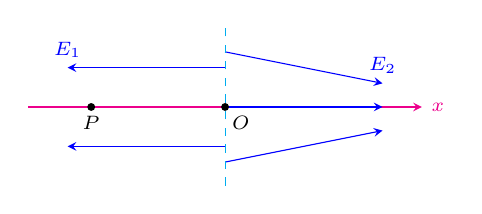
\begin{tikzpicture}[>=stealth,font=\scriptsize]
	\draw[->,magenta] (-2.5,0)--(2.5,0)node[right]{\(x\)};
	\draw[->,blue] (0,.5)--(-2,.5)node[above]{ \(E_1\)};
	\draw[->,blue] (0,-.5)--(-2,-.5);
	\draw[->,blue] (0,.7)--(2,.3)node[above]{ \(E_2\)};
	\draw[->,blue] (0,-.7)--(2,-.3);
	\draw[->,blue] (0,0)--(2,0);
	\draw[dashed,cyan] (0,-1)--(0,1);
	\fill (0,0) circle(.05) (-1.7,0)node[below]{ \(P\)} circle(.05);
	\node at(.2,-.2){ \(O\)};
\end{tikzpicture}
\begin{choices}
	\item 粒子最大速度为\qty{3}{m/s}
	\item 粒子运动到原点\(O\)右侧最低电势为\qty{-1.6}{V}
	\item 粒子运动的周期为\(\dfrac{4 + \sqrt{5}\pi}{10}\)\qty{}{s}
	\item 粒子向右运动到\(O\)点的最远距离为\(\dfrac{\sqrt{5}}{5}\)\qty{}{m}
\end{choices}
\begin{answer}
	BC\qquad 提示：
\end{answer}